% =====================================================================
%  Privacy-Preserving Medical Record Sharing System
%  Project Report: MedRec baseline and MedRec+ improvements
%  Compile with: pdflatex report.tex   (run twice for references)
% =====================================================================
\documentclass[11pt,a4paper]{article}

\usepackage[a4paper,top=2cm,bottom=2cm,left=2.1cm,right=2.1cm]{geometry}
\usepackage[T1]{fontenc}
\usepackage[utf8]{inputenc}
\usepackage{mathptmx}
\usepackage[scaled=0.92]{helvet}
\usepackage{courier}
\usepackage{microtype}
\usepackage{amsmath,amssymb}
\usepackage{booktabs,tabularx,array,multirow}
\usepackage[table]{xcolor}
\usepackage{graphicx}
\usepackage{enumitem}
\usepackage{caption}
\usepackage{float}
\usepackage{titlesec}
\usepackage{tikz}
\usetikzlibrary{arrows.meta,positioning,fit,backgrounds,shapes.geometric}
\usepackage{pgfplots}
\pgfplotsset{compat=1.17}
\usepackage[hidelinks]{hyperref}

% ---------- colours and styles ----------
\definecolor{base}{HTML}{8A8F98}
\definecolor{plus}{HTML}{1F6FB2}
\definecolor{accent}{HTML}{B5462E}
\definecolor{soft}{HTML}{EEF3F9}

\titleformat{\section}{\large\bfseries\color{plus}}{\thesection.}{0.5em}{}
\titleformat{\subsection}{\normalsize\bfseries}{\thesubsection}{0.5em}{}
\titlespacing*{\section}{0pt}{9pt}{4pt}
\titlespacing*{\subsection}{0pt}{6pt}{2pt}

\setlist{nosep,leftmargin=1.3em}
\captionsetup{font=small,labelfont=bf,skip=4pt}
\setlength{\parskip}{3pt}
\setlength{\parindent}{0pt}
\sloppy
\renewcommand{\arraystretch}{1.12}
\newcolumntype{Y}{>{\raggedright\arraybackslash}X}

\begin{document}

% =====================================================================
%  PAGE 1 : TITLE PAGE
% =====================================================================
\begin{titlepage}
\centering
\vspace*{1.2cm}

{\large\scshape Project Report\par}
\vspace{1.0cm}

{\color{plus}\rule{\linewidth}{1.2pt}\par}
\vspace{0.5cm}
{\Huge\bfseries Privacy-Preserving Medical\\[4pt] Record Sharing System\par}
\vspace{0.45cm}
{\Large MedRec+: Encrypted, Pseudonymous and Time-Bound\\ Access Control for Blockchain-Based Health Records\par}
\vspace{0.5cm}
{\color{plus}\rule{\linewidth}{1.2pt}\par}

\vspace{1.4cm}

% ---- Team details (edit names and roll numbers here) ----
{\large\bfseries Submitted by\par}
\vspace{0.4cm}
\begin{tabular}{@{}c l l@{}}
\toprule
\textbf{\#} & \textbf{Name} & \textbf{Roll Number} \\
\midrule
1 & A.Palvash Kumar & S20230010029 \\
2 & A.Naga Venkatesh & S20230010001 \\
3 & M.Jashwanth & S20230010145 \\
\bottomrule
\end{tabular}

\vspace{1.6cm}

\begin{minipage}{0.86\linewidth}
\centering\small
\textbf{Base paper}\\[3pt]
A.~Azaria, A.~Ekblaw, T.~Vieira and A.~Lippman,
``MedRec: Using Blockchain for Medical Data Access and Permission Management,''
\emph{2nd Int.\ Conf.\ on Open and Big Data (OBD)}, 2016, pp.~25--30.\\[8pt]
\textbf{Source of improvement ideas}\\[3pt]
M.~Li, S.~Yu, Y.~Zheng, K.~Ren and W.~Lou,
``Scalable and Secure Sharing of Personal Health Records in Cloud Computing
Using Attribute-Based Encryption,'' \emph{IEEE TPDS}, 24(1), 2013.
\end{minipage}

\vfill
{\large October 2026\par}
\end{titlepage}

% =====================================================================
%  ABSTRACT
% =====================================================================
\begin{center}
\begin{minipage}{0.95\linewidth}
\small\textbf{Abstract:}
MedRec keeps medical records in each hospital's own database and uses Ethereum
smart contracts to hold pointers, integrity hashes and access permissions. We
re-implemented MedRec on a local Hardhat chain with a Node.js gatekeeper and an
SQLite provider database, and showed four weaknesses with scripted demonstrations:
the off-chain records are stored in plaintext, on-chain metadata links patients to
providers, access grants never expire, and there is no emergency access route. We
then built \textbf{MedRec+}, which adds envelope encryption (AES-256-GCM with
X25519 key wrapping), pairwise pseudonyms with salted selector commitments,
time-bound grants with key rotation, and an audited break-glass role. In our
local evaluation, clinical plaintext exposure in the database fell from 100\% to
0\%, on-chain identity attribution fell from 100\% to 0\% in the observer model we
tested, and the extra cost was +3.0\% gas to share a record and under 75\,ms of
cryptography for a 50\,MB record. All 42 automated tests pass.
\end{minipage}
\end{center}

% =====================================================================
\section{Introduction}
% =====================================================================
A patient's medical history is usually spread across several hospitals, clinics
and laboratories, each with its own database. Sharing records between them is
slow, and the patient rarely knows who has seen their data. Central record
repositories solve the fragmentation problem but create a single high-value target
for attackers and require everyone to trust one operator. The cyber security problem
we address is therefore: \emph{how can records be shared between providers under
the patient's control, without exposing them to storage insiders, to observers of
the sharing system, or to people whose access should have ended?}

Putting records directly on a blockchain does not solve this. A public ledger is
readable by every node, it cannot erase data (which conflicts with privacy
regulation), and storing large files on-chain is very expensive. The design space
is therefore ``data off-chain, permissions on-chain'', which is exactly what MedRec
proposes. Our objectives were to (i) re-implement MedRec faithfully, (ii) find and
demonstrate its limitations, (iii) design and implement improvements, and (iv)
measure their benefit and cost against the baseline.

\subsection{Why we selected this paper}
We shortlisted two well-cited papers on the topic and scored them on six criteria
(1 = poor, 5 = strong). Table~\ref{tab:select} summarises the comparison.

\begin{table}[H]
\centering\small
\caption{Paper selection: MedRec versus Li et al.\ (attribute-based encryption for PHRs).}
\label{tab:select}
\begin{tabularx}{\linewidth}{@{}Ycc@{}}
\toprule
\textbf{Criterion} & \textbf{MedRec (2016)} & \textbf{Li et al.\ (2013)} \\
\midrule
Implementable by a student team in 4--5 weeks & 5 & 2 \\
Mainstream tooling that installs cleanly & 5 & 2 \\
Produces measurable results (gas, latency, throughput) & 4 & 4 \\
Limitations are clearly stated and citable & 5 & 4 \\
Room for a meaningful, implementable improvement & 5 & 4 \\
Fit with a JavaScript stack (Hardhat, Node.js) & 5 & 2 \\
\midrule
\textbf{Total (out of 30)} & \textbf{29} & \textbf{18} \\
\bottomrule
\end{tabularx}
\end{table}

We chose \textbf{MedRec} for three reasons. First, it is buildable: three smart
contracts, a gatekeeper service and a database can be implemented, tested and
benchmarked in a few weeks, whereas a faithful reproduction of Li et al.\ needs
pairing-based cryptography, multi-authority ABE and proxy re-encryption. Second,
the authors themselves point to the gaps: contract-level encryption was not added
to the prototype, no encryption of the off-chain data is described, and they
acknowledge that transaction patterns remain open to forensic analysis. That gave
us a well-defined improvement target. Third, MedRec reports no performance
evaluation (it lists simulation of system efficiency as future work), so our
measurements add something new. We used Li et al.\ not as a system to rebuild but
as the source of three ideas: encrypting each file under its own random key,
break-glass emergency access, and deferring re-encryption on revocation.

% =====================================================================
\section{Overview of the Existing Technique (MedRec)}
% =====================================================================
MedRec separates \emph{where data lives} from \emph{who may see it}. Records stay
in the provider's own database behind a \emph{gatekeeper} server. The blockchain
stores only small items: a pointer to the record, a hash that proves it has not
been changed, and the list of addresses allowed to view it. Three contracts
implement this (Table~\ref{tab:contracts}).

\begin{table}[H]
\centering\small
\caption{MedRec smart contracts.}
\label{tab:contracts}
\begin{tabularx}{\linewidth}{@{}l Y@{}}
\toprule
\textbf{Contract} & \textbf{Role} \\
\midrule
Registrar (RC) & Maps a participant's identity string (name or ID) to an Ethereum address and to their Summary contract. \\
Summary (SC) & Per-participant index of every patient--provider relationship, with a status flag used for notifications. \\
Patient--Provider Relationship (PPR) & One per relationship. Holds data pointers (query selector + hash), the gatekeeper location and viewer permissions. \\
\bottomrule
\end{tabularx}
\end{table}

\textbf{Workflow:} (1) A provider adds a record to its database and calls
\texttt{addPointer} on the PPR with the record's selector and hash. (2) The
patient's Summary contract is flagged, so the patient sees the new record. (3) The
patient calls \texttt{share} to permit a doctor or lab. (4) The viewer sends a
signed request to the gatekeeper, which checks \texttt{canView} on-chain, runs the
query and returns the record; the viewer checks the hash against the on-chain value.
The approach gives the patient a single view of all relationships, an immutable
permission history and no central data store. Figure~\ref{fig:arch} shows the
architecture, with a summary of the MedRec+ changes.

\begin{figure}[H]
\centering
\begin{tikzpicture}[
  font=\small,
  box/.style={draw,rounded corners=2pt,align=center,minimum height=0.95cm,minimum width=2.2cm,inner sep=3pt,fill=white},
  arr/.style={-{Stealth[length=2.2mm]},thick},
  lab/.style={font=\scriptsize,fill=white,inner sep=1pt}
]
% blockchain row
\node[box] (rc)  at (0,0)   {Registrar\\[-2pt]\scriptsize names $\to$ addresses};
\node[box] (sc)  at (3.4,0) {Summary\\[-2pt]\scriptsize relationship list};
\node[box] (ppr) at (6.8,0) {PPR\\[-2pt]\scriptsize pointers, hashes,\\[-3pt]\scriptsize permissions};
\begin{scope}[on background layer]
\node[draw=plus,dashed,rounded corners,fill=soft,fit=(rc)(sc)(ppr),inner sep=6pt,
      label={[font=\small\bfseries,text=plus]above:Ethereum smart contracts (local Hardhat chain)}] (chain) {};
\end{scope}
% off-chain row
\node[box] (pat) at (0,-2.7)   {Patient\\[-2pt]\scriptsize wallet};
\node[box] (vw)  at (3.4,-2.7) {Doctor / Viewer\\[-2pt]\scriptsize wallet};
\node[box] (gk)  at (6.8,-2.7) {Gatekeeper\\[-2pt]\scriptsize Node.js};
\node[box] (db)  at (10.4,-2.7) {Provider DB\\[-2pt]\scriptsize SQLite};
\node[box] (prov) at (10.4,0)  {Provider\\[-2pt]\scriptsize wallet};
% arrows
\draw[arr] (pat) -- node[lab,align=center]{register,\\ share, revoke} (pat |- chain.south);
\draw[arr] (vw) -- node[lab,above=1pt]{signed} node[lab,below=1pt]{request} (gk);
\draw[arr] (gk) -- node[lab]{canView()} (gk |- chain.south);
\draw[arr] (gk) -- node[lab,above=1pt]{query} (db);
\draw[arr] (prov) -- node[lab,above=2pt]{addPointer} (chain.east |- prov);
\draw[arr,dashed] (gk.south) -- ++(0,-0.5) -| node[pos=0.25,lab,below=1pt]{record returned; viewer checks hash} (vw.south);
% MedRec+ legend
\node[draw=plus,rounded corners=2pt,fill=soft,text width=3.05cm,align=left,font=\scriptsize,inner sep=4pt,anchor=north west]
  (leg) at (12.0,0.75) {\hyphenpenalty=10000\exhyphenpenalty=10000\textbf{\color{plus}MedRec+ changes}\\[2pt]
  \textbullet\ Registrar: no names, stores X25519 key only\\
  \textbullet\ PPR: $H(\mathit{sel}\Vert\mathit{salt})$, expiry, revoke flag, break-glass\\
  \textbullet\ New events: KeyWrapped, EmergencyAccess\\
  \textbullet\ Pairwise pseudonymous patient addresses\\
  \textbullet\ DB holds \mbox{AES-256-GCM} ciphertext only};
\end{tikzpicture}
\caption{MedRec architecture as we implemented it. The box on the right lists what MedRec+ changes.}
\label{fig:arch}
\end{figure}

% =====================================================================
\section{Implementation of the Existing Approach}
% =====================================================================
\textbf{Stack:} Contracts are written in Solidity~0.8.24 and run on a local Hardhat~2
chain; tests use Mocha through \texttt{hardhat-toolbox}; clients and the gatekeeper
use Node.js with \texttt{ethers}~v6, Express~5 and \texttt{better-sqlite3}. The
provider database holds six synthetic patient records (name, date of birth, blood
type, diagnosis, medication, visit date); no real patient data was used.

\textbf{Components built:} The three contracts (\texttt{Registrar.sol},
\texttt{Summary.sol}, \texttt{PPR.sol}) follow the paper. A command-line client
(\texttt{client/cli.js}) implements the add-record, retrieve and share flows for
patient, provider and viewer, and a gatekeeper service (\texttt{gatekeeper/index.js})
verifies each request. The gatekeeper recovers the
signer from a signed \{PPR, selector, nonce, timestamp\} message, rejects reused
nonces and stale timestamps (replay protection), calls \texttt{canView} on-chain,
runs a parameterised query, and compares the SHA-256 of the result with the on-chain
hash before returning it.

\textbf{Deviations, stated honestly:} (a) MedRec stores raw query strings on-chain
and the gatekeeper executes them; running query text taken from a public
transaction invites SQL injection, so we used selectors mapped to parameterised
queries. (b) Proof-of-work mining and the researcher ``bounty'' model were
replaced by a local chain with emulated block times (instant, 2\,s and 12\,s).
(c) Identity strings were kept on-chain as in the paper, because that is one of the
behaviours we later critique.

\textbf{Baseline results:} 21 automated tests pass (15 contract tests and 6
gatekeeper integration tests covering authorisation, replay and tampering). Over
30 runs, registration cost 336,401 gas on average and a record pointer used 132
bytes of calldata. Transaction latency was 0.67\,ms with instant mining but
2,014.6\,ms and 12,011.9\,ms at 2\,s and 12\,s block intervals, so confirmation time
is set by the consensus interval rather than by contract execution. The gatekeeper
served up to 509 requests/s with 100 concurrent clients, with no errors.

% =====================================================================
\section{Challenges and Limitations}
% =====================================================================
We scripted four weakness demonstrations (D1--D4) against our baseline. Together
with the authors' own stated limitations they give the challenges in
Table~\ref{tab:challenges}.

\begin{table}[H]
\centering\small
\caption{Challenges found in MedRec, with evidence and impact.}
\label{tab:challenges}
\begin{tabularx}{\linewidth}{@{}>{\raggedright\arraybackslash}p{2.5cm} Y Y@{}}
\toprule
\textbf{Challenge} & \textbf{Evidence} & \textbf{Security impact} \\
\midrule
C1 Plaintext off-chain data &
D1: opening the SQLite file shows 6/6 records in clear text. D4: calling the data layer directly bypasses the contract check. &
A database dump, an insider or a compromised gatekeeper exposes every record. Protection depends on server code, not cryptography. \\
\addlinespace
C2 Linkable on-chain metadata &
D2: an observer script reads Registrar names, PPR links, viewer lists and selectors such as \texttt{records:oncology}. &
Anyone running a node learns who is treated where, who was given access and hints about the condition (100\% attribution). \\
\addlinespace
C3a No expiry on access &
Grants last until manually revoked; the paper only suggests expiry. D3: a revoked viewer keeps data already fetched. &
A previous doctor keeps standing access after treatment ends. \\
\addlinespace
C3b No emergency route &
No mechanism for access without a prior grant. &
An unconscious patient's allergies or blood group cannot be released in time. \\
\addlinespace
C4 Scalability &
Listed as unresolved by the authors; latency follows block time (12\,s per confirmation). &
Measured and discussed only; not addressed by our design. \\
\bottomrule
\end{tabularx}
\end{table}

% =====================================================================
\section{Proposed Approach: MedRec+}
% =====================================================================
\textbf{Threat model:} We defend against four adversaries: A1, a curious storage
operator who can read the database but holds no keys; A2, a passive chain observer
who reads all state, calldata and events; A3, a revoked or expired viewer who tries
to fetch again; and A4, an impostor claiming an emergency. The provider that
creates a record is a trusted custodian, and endpoint malware and network traffic
analysis are out of scope. Our design goal was to fix C1--C3 with standard,
fast cryptography rather than heavy ABE.

\textbf{E1 -- Envelope encryption (fixes C1):} Each record is encrypted with a
fresh 256-bit data encryption key (DEK) using AES-256-GCM, with the record ID bound
as authenticated associated data (AAD) so a ciphertext cannot be swapped onto
another record. The DEK is then \emph{wrapped} separately for each authorised
reader: an ephemeral X25519 key agreement with the reader's public key, HKDF-SHA256
to derive a wrapping key, and AES-GCM to encrypt the DEK. Only ciphertext reaches
the database; the on-chain hash is the SHA-256 of the ciphertext. Wrapped keys are
published as \texttt{KeyWrapped} contract events rather than in storage, which we
show is much cheaper.

\begin{figure}[H]
\centering
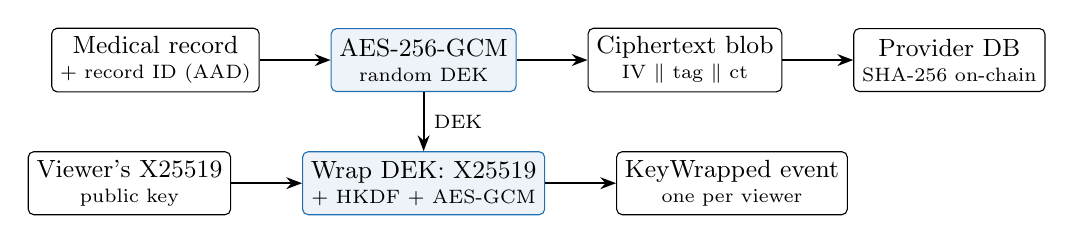
\begin{tikzpicture}[font=\small,
  b/.style={draw,rounded corners=2pt,align=center,minimum height=0.8cm,inner sep=3pt},
  k/.style={b,fill=soft,draw=plus},
  arr/.style={-{Stealth[length=2mm]},thick}]
\node[b] (rec) {Medical record\\[-2pt]\scriptsize + record ID (AAD)};
\node[k,right=0.9cm of rec] (aes) {AES-256-GCM\\[-2pt]\scriptsize random DEK};
\node[b,right=0.9cm of aes] (blob) {Ciphertext blob\\[-2pt]\scriptsize IV $\Vert$ tag $\Vert$ ct};
\node[b,right=0.9cm of blob] (db) {Provider DB\\[-2pt]\scriptsize SHA-256 on-chain};
\node[k,below=0.75cm of aes] (wrap) {Wrap DEK: X25519\\[-2pt]\scriptsize + HKDF + AES-GCM};
\node[b,right=0.9cm of wrap] (ev) {KeyWrapped event\\[-2pt]\scriptsize one per viewer};
\node[b,left=0.9cm of wrap] (pk) {Viewer's X25519\\[-2pt]\scriptsize public key};
\draw[arr] (rec) -- (aes); \draw[arr] (aes) -- (blob); \draw[arr] (blob) -- (db);
\draw[arr] (aes) -- node[right,font=\scriptsize]{DEK} (wrap);
\draw[arr] (pk) -- (wrap); \draw[arr] (wrap) -- (ev);
\end{tikzpicture}
\caption{E1 envelope encryption: bulk data under a per-record key, the key wrapped per reader.}
\label{fig:envelope}
\end{figure}


\textbf{E2 -- Reduced linkability (fixes C2):} \texttt{RegistrarPlus} stores no
identity strings. A patient uses a separate pseudonymous address for each provider
relationship, so relationships cannot be joined by address. Selectors are stored as
salted commitments $c = \mathrm{SHA256}(\mathit{selector}\,\Vert\,\mathit{salt})$,
with the salt shared only with the counterparty, so an observer sees an opaque
32-byte value instead of ``records:cardiology''.

\textbf{E3 -- Time-bound grants and key rotation (fixes C3a):} A grant is now
\{viewer, selector commitment, \texttt{expiresAt}, \texttt{revoked}\}, and
\texttt{canView} returns true only if \texttt{block.timestamp < expiresAt} and the
grant is not revoked. When a record is updated after a revocation, a new DEK is
generated and wrapped only for the remaining viewers, so a revoked viewer cannot
decrypt future versions even if they obtain the ciphertext.

\textbf{E4 -- Audited break-glass (fixes C3b):} The patient designates an emergency
role (e.g.\ an emergency department) and flags a minimal emergency record set
(allergies, blood group, medication). Only that role can call
\texttt{emergencyAccess}, which requires a duration between 1 second and 24 hours,
sets an automatic expiry and emits a public \texttt{EmergencyAccess} event. Every
use is therefore auditable, and the patient can revoke it afterwards.


% =====================================================================
\section{Implementation of the Proposed Approach}
% =====================================================================
MedRec+ was built alongside the baseline so that the same benchmark harness could
run both modes. Table~\ref{tab:impl} lists what changed.

\begin{table}[H]
\centering\small
\caption{Implementation of the MedRec+ enhancements.}
\label{tab:impl}
\begin{tabularx}{\linewidth}{@{}p{4.0cm} Y@{}}
\toprule
\textbf{File} & \textbf{What it implements} \\
\midrule
\texttt{crypto-envelope.js} & E1: \texttt{encryptRecord}, \texttt{wrapKey}, \texttt{unwrapKey}, \texttt{decryptRecord} and \texttt{computeSelectorCommit}, built only on Node's \texttt{crypto} module (no third-party crypto). Ciphertext adds a constant 28 bytes (12-byte IV + 16-byte tag). \\
\texttt{RegistrarPlus.sol} & E2: registration by address and X25519 public key only; no identity strings. \\
\texttt{PPRPlus.sol} & E1--E4: pointers keyed by selector commitments with timestamps; \texttt{Grant} struct with expiry and revoked flag; \texttt{share} (event) and \texttt{shareWithStorage} (for comparison); O(1) \texttt{revoke}; emergency role, emergency selector set and \texttt{emergencyAccess} with a 24-hour cap. \\
\texttt{gatekeeper/index.js} & Dual mode: in MedRec+ mode it checks the grant on-chain, returns only ciphertext from the \texttt{records\_encrypted} table and resolves the caller's wrapped key from events. \\
\texttt{deploy-plus.js} & Seeds an encrypted database with no clinical plaintext columns and deploys the MedRec+ contracts. \\
\texttt{medrec-plus.test.js} & 21 tests: registration, pointers, grants, expiry, revocation, break-glass, gatekeeper queries and DEK rotation. \\
Analysis and bench scripts & \texttt{observer-compare.js} (H2) and \texttt{security-experiments.js} (H1, H3--H7), writing CSV/JSON to \texttt{bench/results/}. \\
\bottomrule
\end{tabularx}
\end{table}

The core permission check in \texttt{PPRPlus.sol} shows how E3 and E4 combine:

\begin{footnotesize}
\begin{verbatim}
function canView(address who, bytes32 selectorCommit) external view returns (bool) {
    if (who == patient || who == provider) return true;
    if (who == emergencyRole && emergencyRole != address(0) &&
        block.timestamp < emergencyExpiresAt && emergencySelectors[selectorCommit])
        return true;                                   // E4: audited break-glass
    Grant memory g = grants[who][selectorCommit];
    if (!g.exists || g.revoked) return false;          // E3: explicit revocation
    return block.timestamp < g.expiresAt;              // E3: automatic expiry
}
\end{verbatim}
\end{footnotesize}

The full regression suite now has \textbf{42 tests} (15 baseline contract, 6
gatekeeper integration and 21 MedRec+), all passing in about 620\,ms via
\texttt{npm test}.

% =====================================================================
\section{Results and Analysis}
% =====================================================================
We tested seven hypotheses (H1--H7) with the same harness for both systems.
Table~\ref{tab:results} gives the security results and Figures~\ref{fig:gas}--\ref{fig:tput}
the costs. Gas values are transaction receipts under identical chain state.

\begin{table}[H]
\centering\small
\caption{Security results: baseline MedRec versus MedRec+.}
\label{tab:results}
\begin{tabularx}{\linewidth}{@{}l Y Y@{}}
\toprule
\textbf{Hypothesis / metric} & \textbf{Baseline MedRec} & \textbf{MedRec+} \\
\midrule
H1 Clinical plaintext in DB & 100\% readable (6/6) & \textbf{0\% readable (0/6)} \\
H2 On-chain identity attribution & 100\% & \textbf{0\% (0/3)} in our observer model \\
H2 Plaintext selectors leaked & 2 & \textbf{0} (salted commitments) \\
H2 Largest address cluster & 2 relationships & \textbf{1} (pairwise pseudonyms) \\
H5 Access after expiry / revoke & No expiry exists & \textbf{100\% blocked}, 0 leaks \\
H6 Break-glass auditability & Not supported & \textbf{100/100} events logged \\
H7 Tamper: flipped ciphertext byte & SHA-256 mismatch only & \textbf{Rejected} by GCM and hash \\
H7 Tamper: record swapped to other ID & Not detected & \textbf{Rejected} by AAD \\
\bottomrule
\end{tabularx}
\end{table}

\begin{figure}[H]
\centering
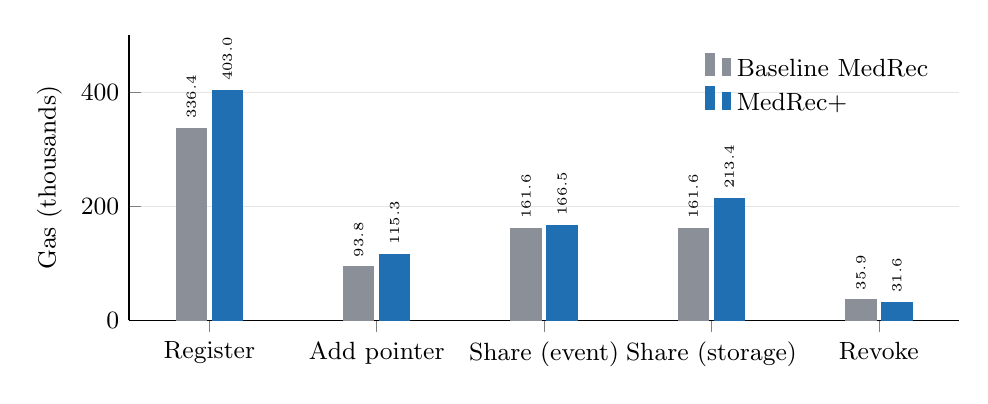
\begin{tikzpicture}
\begin{axis}[
  ybar, bar width=11pt, width=\linewidth, height=5.2cm,
  ymin=0, ymax=500, ylabel={Gas (thousands)}, ylabel style={font=\small},
  symbolic x coords={Register,Add pointer,Share (event),Share (storage),Revoke},
  xtick=data, tick label style={font=\small},
  nodes near coords, nodes near coords style={font=\tiny,rotate=90,anchor=west,/pgf/number format/fixed,/pgf/number format/precision=1,/pgf/number format/fixed zerofill,/pgf/number format/1000 sep={}},
  legend style={at={(0.98,0.96)},anchor=north east,font=\small,draw=none,fill=none},
  legend cell align=left, enlarge x limits=0.12, axis lines*=left, ymajorgrids, grid style={gray!20}]
\addplot[fill=base,draw=base] coordinates {(Register,336.4) (Add pointer,93.8) (Share (event),161.6) (Share (storage),161.6) (Revoke,35.9)};
\addplot[fill=plus,draw=plus] coordinates {(Register,403.0) (Add pointer,115.3) (Share (event),166.5) (Share (storage),213.4) (Revoke,31.6)};
\legend{Baseline MedRec, MedRec+}
\end{axis}
\end{tikzpicture}
\caption{Gas per operation (H4). Creating a PPR, not shown, rose from 1,160,475 to 1,268,715 gas (+9.3\%).}
\label{fig:gas}
\end{figure}

\textbf{Gas (H4):} Registration costs 19.8\% more because the X25519 public key is
stored, and adding a pointer 22.9\% more for the commitment and timestamp. Sharing
is the most frequent operation, and publishing the wrapped key as an event keeps
its overhead to \textbf{+3.0\%} (166,498 gas); writing it to storage would cost
+32.0\%. Storage is therefore 46,862 gas (28.1\%) more expensive than events.
Revocation became \textbf{12.0\% cheaper} because it sets a single flag instead of
shifting an array.

\begin{figure}[H]
\centering
\begin{minipage}[t]{0.49\linewidth}
\centering
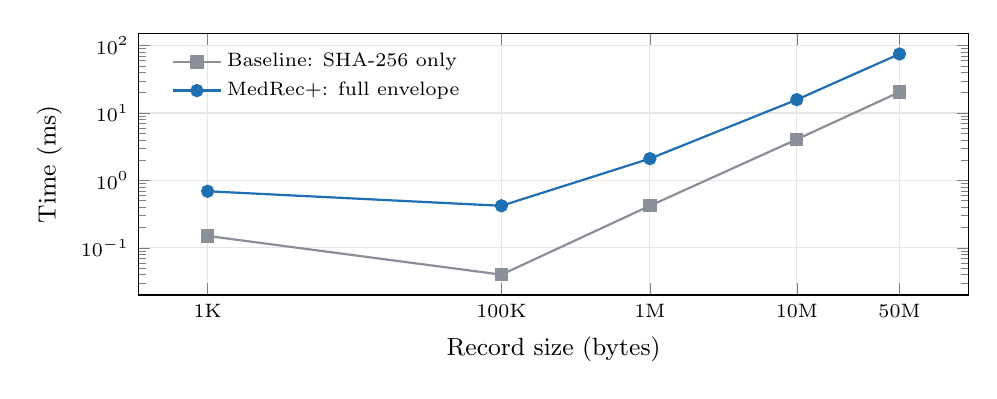
\begin{tikzpicture}
\begin{loglogaxis}[
  width=\linewidth, height=4.9cm,
  xlabel={Record size (bytes)}, ylabel={Time (ms)}, label style={font=\small},
  xtick={1,100,1024,10240,51200}, xticklabels={1K,100K,1M,10M,50M},
  tick label style={font=\scriptsize}, ymin=0.02, ymax=150,
  legend style={at={(0.03,0.97)},anchor=north west,font=\scriptsize,draw=none,fill=none},
  legend cell align=left, grid=major, grid style={gray!20}]
\addplot[base,thick,mark=square*] coordinates {(1,0.15) (100,0.04) (1024,0.42) (10240,4.06) (51200,20.39)};
\addplot[plus,thick,mark=*] coordinates {(1,0.69) (100,0.42) (1024,2.10) (10240,15.74) (51200,74.97)};
\legend{Baseline: SHA-256 only, MedRec+: full envelope}
\end{loglogaxis}
\end{tikzpicture}
\caption{Cryptographic time vs.\ record size (H3).}
\label{fig:lat}
\end{minipage}\hfill
\begin{minipage}[t]{0.49\linewidth}
\centering
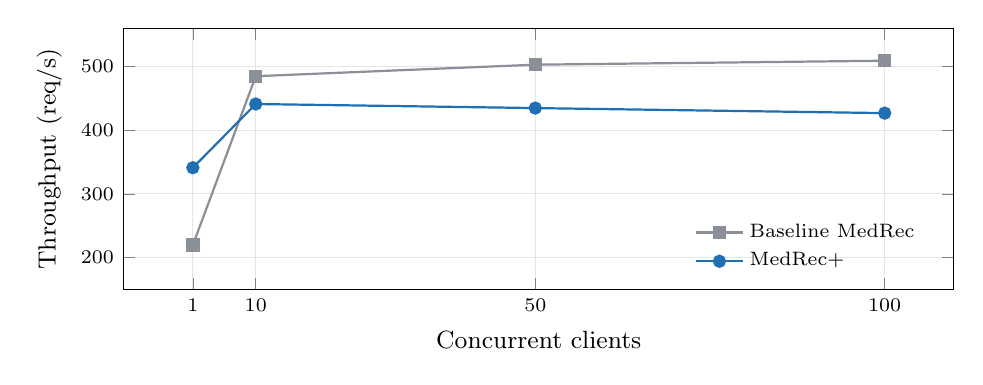
\begin{tikzpicture}
\begin{axis}[
  width=\linewidth, height=4.9cm,
  xlabel={Concurrent clients}, ylabel={Throughput (req/s)}, label style={font=\small},
  xtick={1,10,50,100}, tick label style={font=\scriptsize}, ymin=150, ymax=560,
  legend style={at={(0.97,0.03)},anchor=south east,font=\scriptsize,draw=none,fill=none},
  legend cell align=left, grid=major, grid style={gray!20}]
\addplot[base,thick,mark=square*] coordinates {(1,219.8) (10,484.7) (50,502.8) (100,509.0)};
\addplot[plus,thick,mark=*] coordinates {(1,341.1) (10,441.1) (50,434.7) (100,426.8)};
\legend{Baseline MedRec, MedRec+}
\end{axis}
\end{tikzpicture}
\caption{Gatekeeper throughput (B4).}
\label{fig:tput}
\end{minipage}
\end{figure}

\textbf{Latency and throughput (H3, B4):} The full envelope (encrypt, wrap, unwrap,
decrypt) took 0.69\,ms for 1\,KB, 2.10\,ms for 1\,MB and 74.97\,ms for 50\,MB, with a
fixed 28-byte ciphertext expansion. The baseline line measures only the SHA-256
hash, so the gap is a comparison of two different workloads rather than a pure
overhead; sub-millisecond baseline points are within timer noise. Either way, the
cost is tiny next to a 12\,s block confirmation. Under 100 concurrent clients the
MedRec+ gatekeeper served 426.8\,req/s against 509.0 for the baseline (p95 latency
304.9\,ms versus 229.9\,ms), a 16\% reduction caused by key resolution and
commitment checks; with one client MedRec+ was faster because it looks records up
by primary key. No request failed in either mode.

\begin{table}[H]
\centering\small
\caption{Feature summary: what the improvement changes.}
\label{tab:features}
\begin{tabularx}{\linewidth}{@{}l Y Y@{}}
\toprule
\textbf{Feature} & \textbf{Baseline MedRec} & \textbf{MedRec+} \\
\midrule
Off-chain record storage & Plaintext in SQLite & AES-256-GCM ciphertext, per-record DEK \\
Identity on chain & Names in Registrar & Pairwise pseudonymous addresses \\
Query selectors on chain & Readable text & Salted SHA-256 commitments \\
Access expiry & None & On-chain \texttt{expiresAt}, checked every request \\
After revocation & Old access path only & DEK rotation for new versions \\
Emergency access & Not supported & Role-restricted, max 24\,h, public audit event \\
Tamper detection & SHA-256 hash & SHA-256 + GCM tag + record-ID binding \\
Automated tests & 21 & 42 (all passing) \\
\bottomrule
\end{tabularx}
\end{table}

\textbf{Discussion:} MedRec+ removes the two largest privacy leaks of MedRec at a
moderate, predictable cost. Some exposure remains, and we report it plainly: the
database still shows patient IDs, timestamps and ciphertext lengths; pseudonymous
addresses can be linked if they are funded from one wallet or timed with a visit;
\texttt{Shared} events still show that two addresses interacted; revocation cannot
recall data already decrypted; and the 0\% attribution figure holds for our
simulated observer, not for every possible re-identification attack.

% =====================================================================
\section{Conclusion}
% =====================================================================
We re-implemented MedRec, demonstrated that its off-chain records are plaintext,
its on-chain metadata is linkable, and its grants neither expire nor allow
emergency access, and then built MedRec+ to address these gaps with standard
primitives. In our local evaluation MedRec+ cut database plaintext exposure from
100\% to 0\% and on-chain identity attribution from 100\% to 0\%, enforced expiry
and revocation with zero leaks, logged every emergency access, and detected all
tampering, while adding only 3.0\% gas to sharing and under 75\,ms of cryptography
for a 50\,MB record. Future work includes patient key recovery (social recovery or
provider escrow), proxy re-encryption so that sharing does not require the patient
to unwrap the key, attribute-based policies, zero-knowledge access proofs to hide
who shares with whom, and evaluation on a public testnet.

% =====================================================================
\begin{thebibliography}{9}
\setlength{\itemsep}{0pt}\small
\bibitem{medrec} A.~Azaria, A.~Ekblaw, T.~Vieira and A.~Lippman, ``MedRec: Using Blockchain for Medical Data Access and Permission Management,'' in \emph{Proc.\ 2nd Int.\ Conf.\ on Open and Big Data (OBD)}, 2016, pp.~25--30, doi:10.1109/OBD.2016.11.
\bibitem{li} M.~Li, S.~Yu, Y.~Zheng, K.~Ren and W.~Lou, ``Scalable and Secure Sharing of Personal Health Records in Cloud Computing Using Attribute-Based Encryption,'' \emph{IEEE Trans.\ Parallel and Distributed Systems}, vol.~24, no.~1, pp.~131--143, 2013, doi:10.1109/TPDS.2012.97.
\bibitem{benaloh} J.~Benaloh, M.~Chase, E.~Horvitz and K.~Lauter, ``Patient Controlled Encryption: Ensuring Privacy of Electronic Medical Records,'' in \emph{Proc.\ ACM Cloud Computing Security Workshop (CCSW)}, 2009.
\bibitem{bmds} J.~Liu, M.~Wu, R.~Sun, X.~Du and M.~Guizani, ``BMDS: A Blockchain-based Medical Data Sharing Scheme with Attribute-Based Searchable Encryption,'' in \emph{Proc.\ IEEE ICC}, 2021, pp.~1--6, doi:10.1109/ICC42927.2021.9500966.
\bibitem{tools} Hardhat, ethers.js v6 and Node.js \texttt{crypto} module documentation (AES-GCM, X25519, HKDF).
\end{thebibliography}

\end{document}
